\input{$UNI_DIR/msc/tex/HWSetup}
\input{$UNI_DIR/msc/tex/EngBindings}

%
% Homework Details
%   - Title
%   - Subtitle
%   - Due date
%   - Due time
%   - Course
%   - Section/Time
%   - Instructor
%   - Author
%

\newcommand{\hmwkTitle}{HW02}
\newcommand{\hmwkSubTitle}{Reference Frames and Ground Tracks}
\newcommand{\hmwkDueDate}{October 11th. 2025}
\newcommand{\hmwkDueTime}{11:59 PM}
\newcommand{\hmwkClass}{ENAE 441 - 0101}
\newcommand{\hmwkClassTime}{09:30 AM}
\newcommand{\hmwkClassInstructor}{Dr. Martin}
\newcommand{\hmwkAuthorName}{\textbf{Vai Srivastava}}
\newcommand{\hmwkCompletionDate}{\today}

\begin{document}

\maketitle

\pagebreak

\begin{hwkProblem}{1}{Reference Frame Conversions} \label{hwk:p01}

	Program the transformations between the following reference frames:
	\begin{enumerate}[label=(\alph*)]
		\item \label{hwk:p01a} Perifocal \( \to \) ECI
		\item \label{hwk:p01b} ECI \( \to \) ECEF
		\item \label{hwk:p01c} ECEF \( \to \) Topocentric
	\end{enumerate}

	\hwkSol{} \label{hwk:s01}

	\hwkPart{} \label{hwk:s01a}

	\inputminted{python}{./code/s01a.txt}

	\hwkPart{} \label{hwk:s01b}

	\inputminted{python}{./code/s01b.txt}

	\hwkPart{} \label{hwk:s01c}

	\inputminted{python}{./code/s01c.txt}

	\hwkCode{} \label{code:s01}

	See the \href{https://www.github.com/vaisriv/enae441-hw02/blob/main/code/hw02.py}{Python code} for this assignment.

\end{hwkProblem}

\begin{hwkProblem}{2}{Orbit in Different Reference Frames} \label{hwk:p02}

	Given the following orbital elements of a satellite:

	\[
		\boldsymbol{X}\left(t_0\right)_{\infty}=\left[\begin{array}{c}
				a      \\
				e      \\
				i      \\
				\omega \\
				\Omega \\
				\theta
			\end{array}\right]=\left[\begin{array}{cc}
				\qty{7e3}{\km}    \\
				0.05              \\
				\qty{45}{\degree} \\
				\qty{30}{\degree} \\
				\qty{60}{\degree} \\
				\qty{0}{\degree}
			\end{array}\right]
	\]

	the gravitational parameter of the Earth \( \mu = \qty{3.986e5}{\km\cubed \per \s\squared} \), and its rotation rate \( \omega_{\mathcal{E}/\mathcal{N}}= \qty{7.2911e-5}{\radian\per\s} \),

	\begin{enumerate}[label=(\alph*)]
		\item \label{hwk:p02a} Plot the trajectory for 24 hours in the following reference frames:
		      \begin{enumerate}[label=(\arabic*)]
			      \item \label{hwk:p02a1} ECI
			      \item \label{hwk:p02a2} Perifocal
			      \item \label{hwk:p02a3} ECEF
		      \end{enumerate}
		      Make sure to label the axes and title each plot.
		\item \label{hwk:p02b} Compare the characteristics of the orbit in the different reference frames. Briefly discuss the advantages and limitations of using each frame to represent the satellite’s orbit.
	\end{enumerate}

	\hwkSol{} \label{hwk:s02}

	\hwkPart{} \label{hwk:s02a}

	\begin{figure}[H] \label{fig:s02a}
		\begin{center}
			\begin{subfigure}{0.3\textwidth} \label{fig:s02a1}
				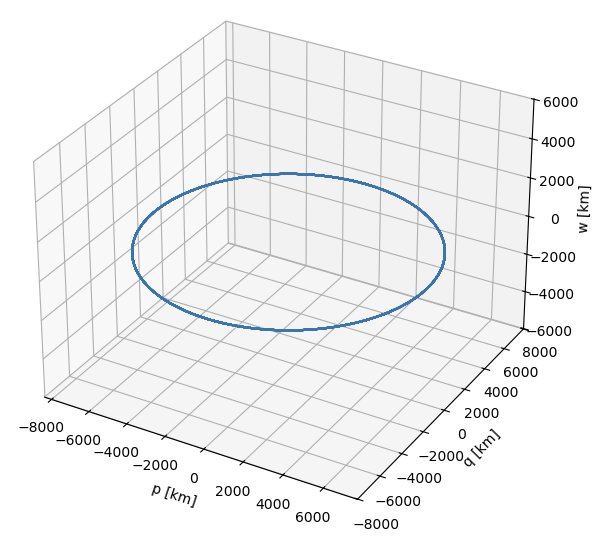
\includegraphics[width=\linewidth]{./images/s02a1.png}
				\caption{Trajectory in Perifocal Frame}
			\end{subfigure}
			\hfill
			\begin{subfigure}{0.3\textwidth} \label{fig:s02a2}
				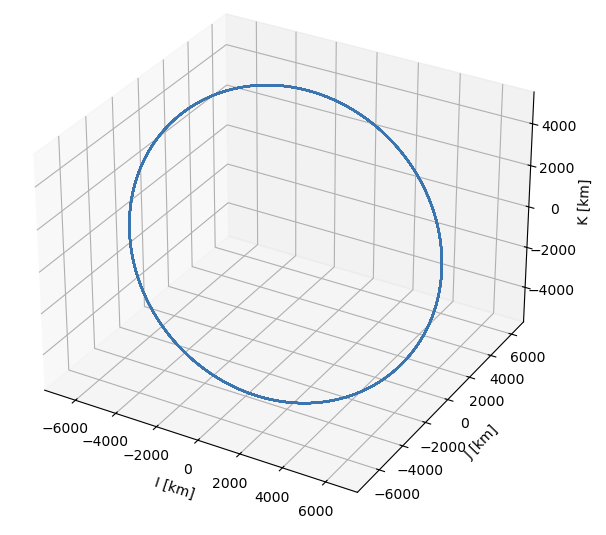
\includegraphics[width=\linewidth]{./images/s02a2.png}
				\caption{Trajectory in ECI Frame}
			\end{subfigure}
			\hfill
			\begin{subfigure}{0.3\textwidth} \label{fig:s02a3}
				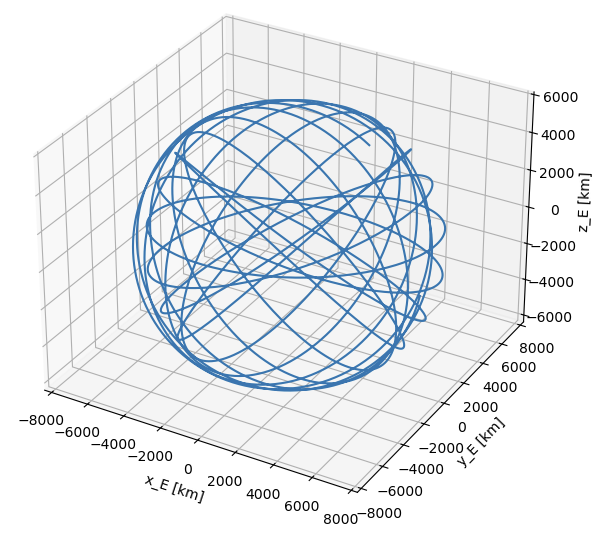
\includegraphics[width=\linewidth]{./images/s02a3.png}
				\caption{Trajectory in ECEF Frame}
			\end{subfigure}
		\end{center}
	\end{figure}

	\hwkPart{} \label{hwk:s02b}

	\inputminted{python}{./code/s02b.txt}

	\hwkCode{} \label{code:s02}

	See the \href{https://www.github.com/vaisriv/enae441-hw02/blob/main/code/hw02.py}{Python code} for this assignment.

\end{hwkProblem}

\begin{hwkProblem}{3}{Ground Tracks of Different Orbits} \label{hwk:p03}

	For each of the following four spacecraft / orbital element sets:

	\[
		\boldsymbol{X}_1=\left[\begin{array}{c}
				a      \\
				e      \\
				i      \\
				\omega \\
				\Omega \\
				\theta
			\end{array}\right] = \left[\begin{array}{cc}
				\qty{6.789e3}{\km}  \\
				0.007               \\
				\qty{51.6}{\degree} \\
				\qty{0}{\degree}    \\
				\qty{215}{\degree}  \\
				\qty{0}{\degree}
			\end{array}\right];
	\]
	\[
		\boldsymbol{X}_2 = \left[\begin{array}{c}
				\qty{26.56e3}{\km} \\
				0.02               \\
				\qty{55}{\degree}  \\
				\qty{0}{\degree}   \\
				\qty{215}{\degree} \\
				\qty{0}{\degree}
			\end{array}\right]; \quad
		\boldsymbol{X}_3=\left[\begin{array}{c}
				\qty{26.6e3}{\km}   \\
				0.74                \\
				\qty{63.4}{\degree} \\
				\qty{270}{\degree}  \\
				\qty{80}{\degree}   \\
				\qty{0}{\degree}
			\end{array}\right]; \quad
		\boldsymbol{X}_4=\left[\begin{array}{c}
				\qty{42.164e3}{\km} \\
				0.00                \\
				\qty{0}{\degree}    \\
				\qty{0}{\degree}    \\
				\qty{35}{\degree}   \\
				\qty{0}{\degree}
			\end{array}\right]
	\]
	\begin{enumerate}[label=(\alph*)]
		\item \label{hwk:p03a} Propagate the orbit for three periods and plot its ground track.
		\item \label{hwk:p03b} Using the ground tracks, identify where the spacecraft is closest to the Earth? A general geographic region is sufficient. Explain.
		\item \label{hwk:p03c} Identify a potential use case for the specific orbit you’ve just plotted. Why might this particular ground track be advantageous?
	\end{enumerate}

	\hwkSol{} \label{hwk:s03}

	\hwkPart{} \label{hwk:s03a}

	\begin{figure}[H] \label{fig:s03a}
		\begin{center}
			\begin{subfigure}{0.4\textwidth} \label{fig:s03a1}
				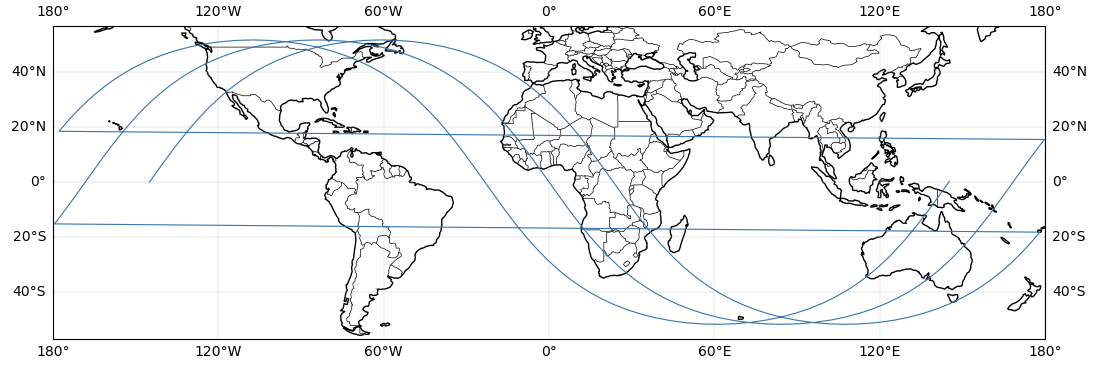
\includegraphics[width=\linewidth]{./images/s03a1.png}
				\caption{X1 (LEO) Ground Track}
			\end{subfigure}
			\begin{subfigure}{0.4\textwidth} \label{fig:s03a2}
				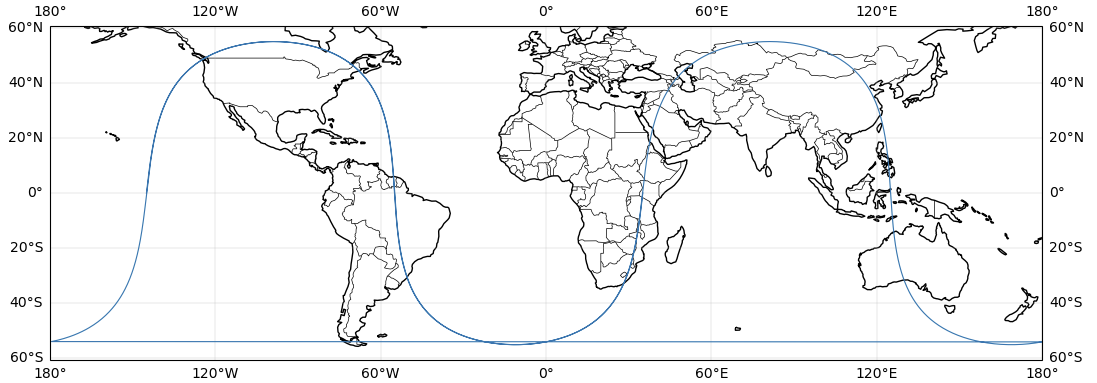
\includegraphics[width=\linewidth]{./images/s03a2.png}
				\caption{X2 (MEO) Ground Track}
			\end{subfigure}
			\\
			\begin{subfigure}{0.4\textwidth} \label{fig:s03a3}
				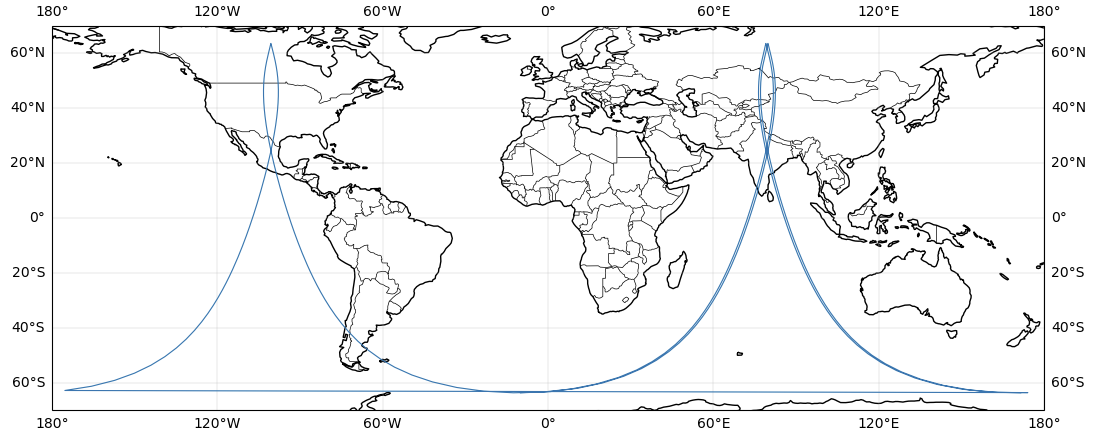
\includegraphics[width=\linewidth]{./images/s03a3.png}
				\caption{X3 (Molniya) Ground Track}
			\end{subfigure}
			\begin{subfigure}{0.4\textwidth} \label{fig:s03a4}
				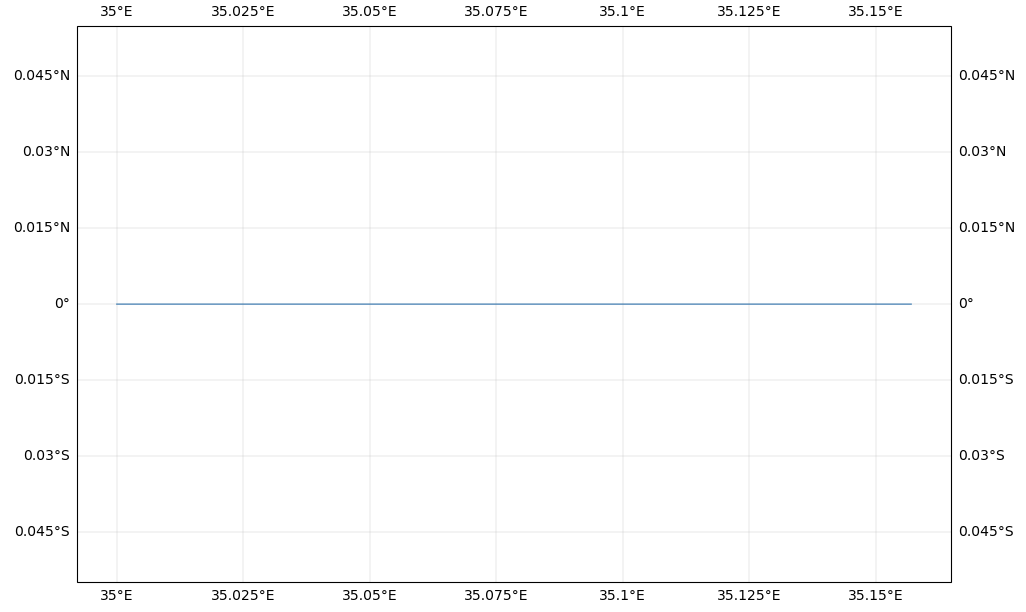
\includegraphics[width=\linewidth]{./images/s03a4.png}
				\caption{X4 (GEO) Ground Track}
			\end{subfigure}
		\end{center}
	\end{figure}

	\hwkPart{} \label{hwk:s03b}

	\inputminted{python}{./code/s03b.txt}

	\hwkPart{} \label{hwk:s03c}

	\inputminted{python}{./code/s03c.txt}

	\hwkCode{} \label{code:s03}

	See the \href{https://www.github.com/vaisriv/enae441-hw02/blob/main/code/hw02.py}{Python code} for this assignment.

\end{hwkProblem}

\begin{hwkProblem}{4}{Measurements from the Deep Space Network Stations} \label{hwk:p04}

	Place an observer at the Goldstone Deep Space Network (DSN) location's latitude and longitude \( \left(\phi, \lambda\right)= \left(\qty{35.2967}{\degree},\qty{-116.9141}{\degree}\right) \). Propagate each spacecraft's trajectory from \hyperref[hwk:p02]{Problem 2} for one orbit:
	\begin{enumerate}[label=(\alph*)]
		\item \label{hwk:p04a} Compute the azimuth and elevation of each spacecraft with respect to the observer. Plot these angular measurements in a polar plot.
		\item \label{hwk:p04b} Compute the range to the spacecraft, and plot the range as a function of time. Be sure to mask any measurements generated when the spacecraft's elevation falls below \qty{10}{\degree}.
		\item \label{hwk:p04c} Interpret the above plots. Which spacecraft are visible to the station at some point along their orbit? Explain.
	\end{enumerate}

	\hwkSol{} \label{hwk:s04}

	\hwkPart{} \label{hwk:s04a}

	\begin{figure}[H] \label{fig:s04a}
		\begin{center}
			\begin{subfigure}{0.4\textwidth} \label{fig:s04a1}
				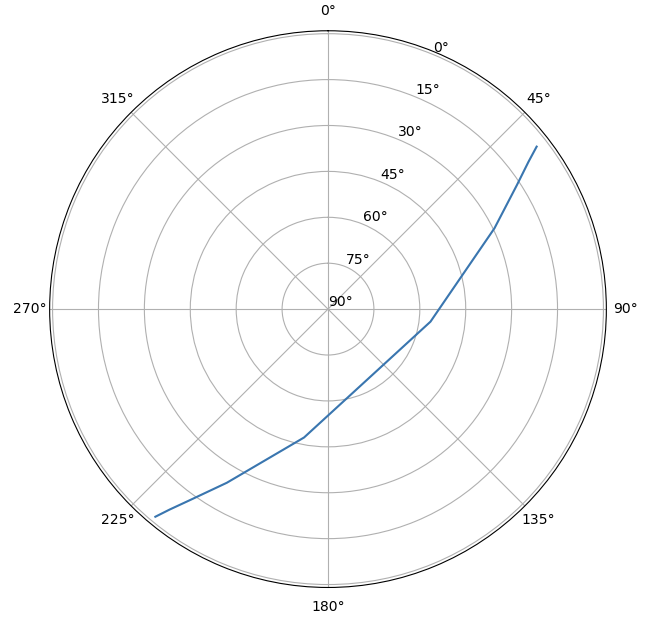
\includegraphics[width=\linewidth]{./images/s04a1.png}
				\caption{X1 (LEO) Azimuth vs. Elevation}
			\end{subfigure}
			\begin{subfigure}{0.4\textwidth} \label{fig:s04a2}
				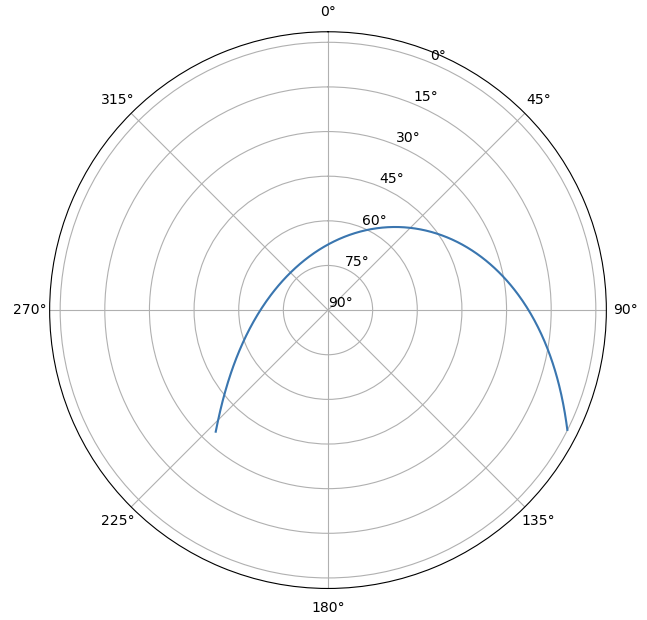
\includegraphics[width=\linewidth]{./images/s04a2.png}
				\caption{X2 (MEO) Azimuth vs. Elevation}
			\end{subfigure}
			\\
			\begin{subfigure}{0.4\textwidth} \label{fig:s04a3}
				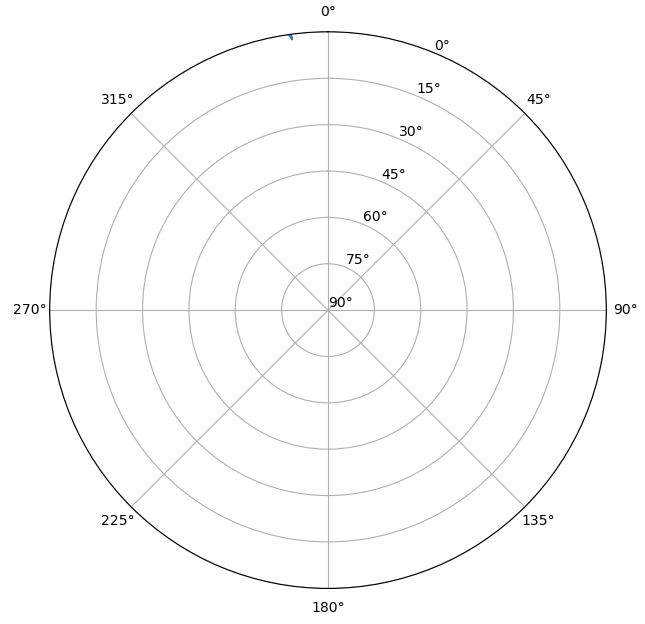
\includegraphics[width=\linewidth]{./images/s04a3.png}
				\caption{X3 (Molniya) Azimuth vs. Elevation}
			\end{subfigure}
			\begin{subfigure}{0.4\textwidth} \label{fig:s04a4}
				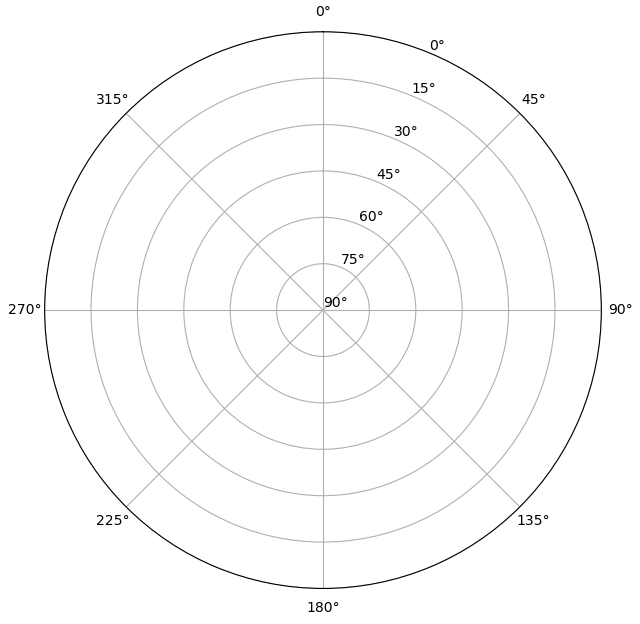
\includegraphics[width=\linewidth]{./images/s04a4.png}
				\caption{X4 (GEO) Azimuth vs. Elevation}
			\end{subfigure}
		\end{center}
	\end{figure}

	\hwkPart{} \label{hwk:s04b}

	\begin{figure}[H] \label{fig:s04b}
		\begin{center}
			\begin{subfigure}{0.4\textwidth} \label{fig:s04b1}
				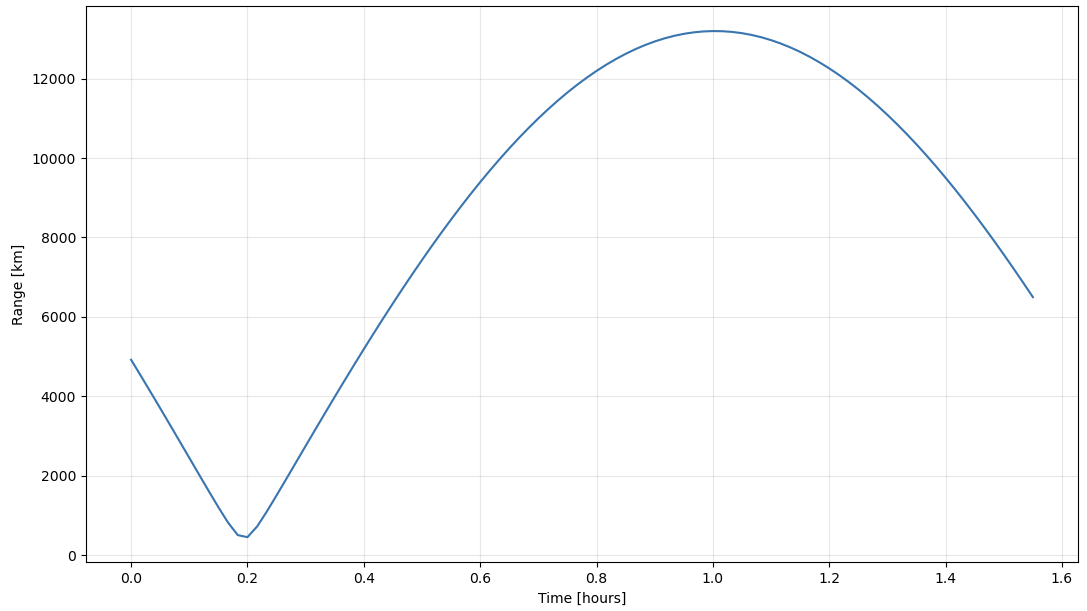
\includegraphics[width=\linewidth]{./images/s04b1.png}
				\caption{X1 (LEO) Range vs. Time}
			\end{subfigure}
			\begin{subfigure}{0.4\textwidth} \label{fig:s04b2}
				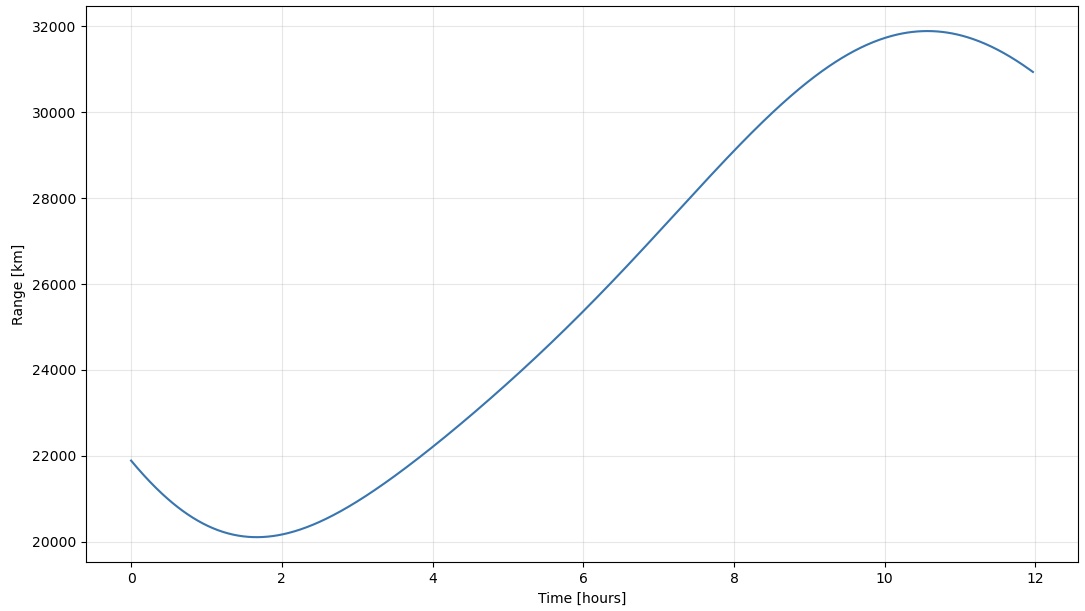
\includegraphics[width=\linewidth]{./images/s04b2.png}
				\caption{X2 (MEO) Range vs. Time}
			\end{subfigure}
			\\
			\begin{subfigure}{0.4\textwidth} \label{fig:s04b3}
				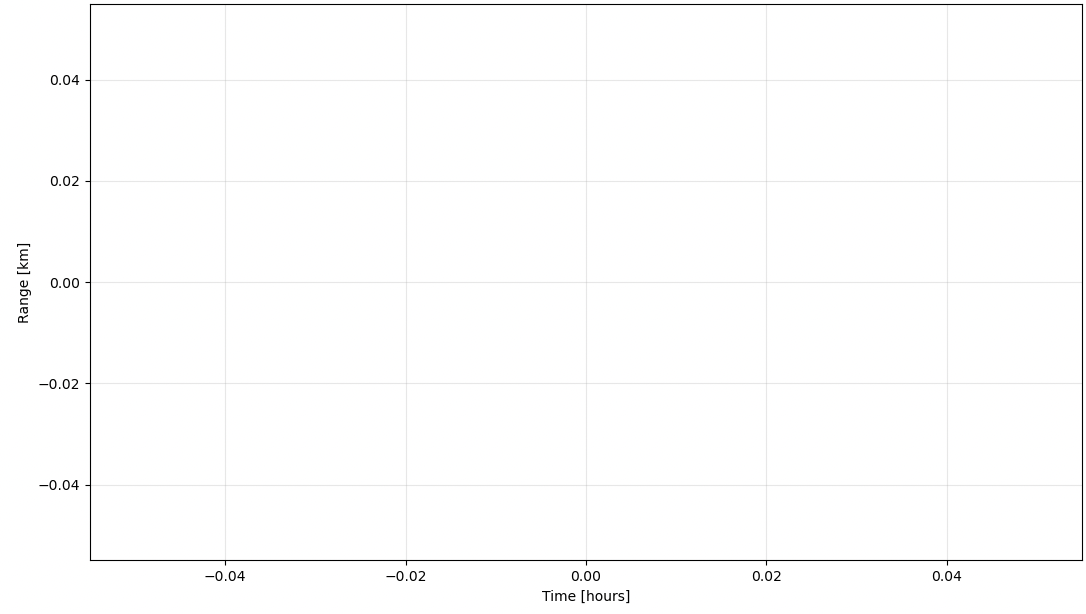
\includegraphics[width=\linewidth]{./images/s04b3.png}
				\caption{X3 (Molniya) Range vs. Time}
			\end{subfigure}
			\begin{subfigure}{0.4\textwidth} \label{fig:s04b4}
				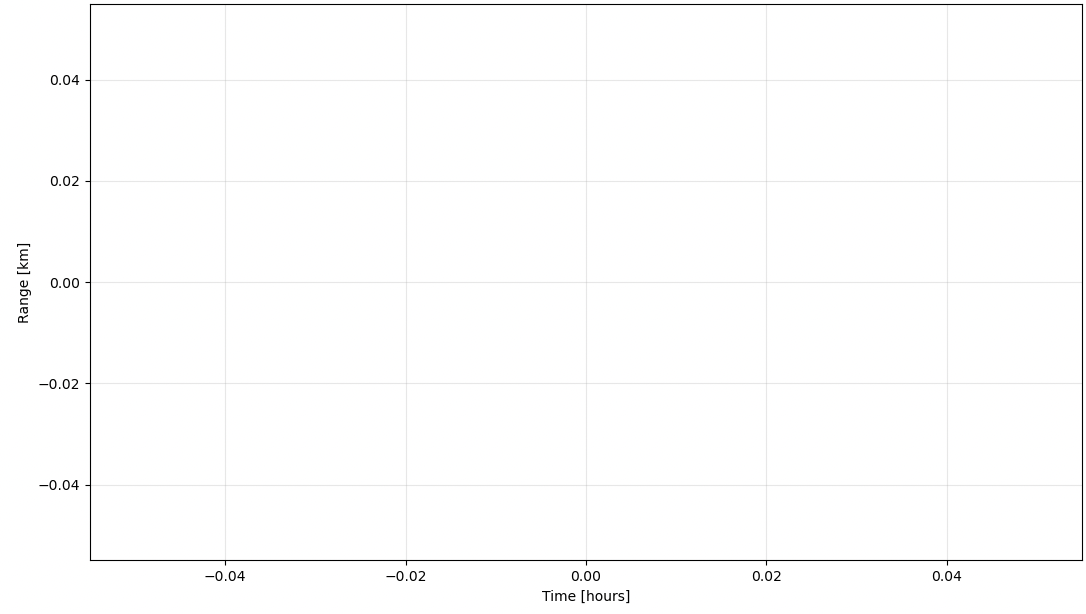
\includegraphics[width=\linewidth]{./images/s04b4.png}
				\caption{X4 (GEO) Range vs. Time}
			\end{subfigure}
		\end{center}
	\end{figure}

	\hwkPart{} \label{hwk:s04c}

	\inputminted{python}{./code/s04c.txt}

	\hwkCode{} \label{code:s04}

	See the \href{https://www.github.com/vaisriv/enae441-hw02/blob/main/code/hw02.py}{Python code} for this assignment.

\end{hwkProblem}

\end{document}
